% Niveau :      PCSI *
% Discipline :  Chimie Orga
% Mots clés :   Stéréochimie

\begin{exercise}{De la cinétique à l'équilibre}{2}{PCSI}
{Transformationn de la matière,Cinétique,Arrhénius}{bermu}

\begin{questions}
\questioncours \'Evolution de la constante de vitesse chimique avec les concentrations et la température.

\begin{EnvUplevel}
    On étudie la réaction d'isomérisation suivante
    $$\mathrm{\underset{\textsfbf{A}}{{CH_3-CO-CH_3}_{(aq)}} \quad\overset{1}{\underset{-1}{\rightleftharpoons}}\quad \underset{\textsfbf{B}}{{CH_3-C(OH)=CH_2}_{(aq)}}},$$
    pour laquelle la constante d'équilibre est $K^\circ$. On introduit initialement \textsfbf{A} avec une concentration $c_0$.
\end{EnvUplevel}

\question Justifier la qualification d'isomérisation.

\question Quel est l'avancement volumique maximal de la réaction $1$, $\xi_\text{max}$ ?

\question Donner les équations cinétiques des vitesses $v_1$ et $v_{-1}$ des deux réactions 1 et $-1$ en fonction des constantes de vitesses $k_1$ et $k_{-1}$.

\question En déduire un système sous la forme
$$\left\lbrace\mqty{\displaystyle\dv{[\textsfbf{A}]}{t} = f\qty\big([\textsfbf{A}],[\textsfbf{B}])\\[2ex] \displaystyle\dv{[\textsfbf{B}]}{t} = g\qty\big([\textsfbf{A}],[\textsfbf{B}])}\right.$$

\question Justifier qualitativement que la concentration totale est constante et donner cette constante. Montrer que le système d'équation précédent vérifie cette propriété.

\question En déduire que l'on peut séparer le système sous la forme
$$\left\lbrace\mqty{\displaystyle\dv{[\textsfbf{A}]}{t} = -\dfrac{1}{\tau}[\textsfbf{A}] + \text{cte}_1 \\[2ex] \displaystyle\dv{[\textsfbf{B}]}{t} = -\dfrac{1}{\tau}[\textsfbf{B}] + \text{cte}_2}\right.$$
On précisera l'expression de $\tau$, cte$_1$ et cte$_2$. Que représente $\tau$ ?

\question On se place à $t \gg \tau$. Décrire l'état final, et en particulier donner l'avancement volumique final $\xi_\text{f}$, le quotient de réaction final $Q_\text{f}$ et les vitesses de réaction $v_1$ et $v_{-1}$. Commentaire ?

\question En déduire une relation entre $K^\circ$, $k_1$ et $k_{-1}$ et lui donner un sens chimique. 

\question Comment évolue $K^\circ$ en fonction de la température ?



\end{questions}


\end{exercise}

% Niveau :      PCSI *
% Discipline :  Chimie Orga
% Mots clés :   Stéréochimie

\begin{exercise}{Modèle clé-serrure de Michaelis--Menten}{3}{PCSI}
{Transformationn de la matière,Cinétique,Arrhénius}{bermu}

\begin{questions}
\questioncours Profil d'énergie potentielle d'une réaction chimique et influence d'un catalyseur.

\begin{EnvUplevel}
     En 1913, à partir de résultats expérimentaux, Victor Henri, Leonor Michaelis et Laure Menten proposent pour une réaction enzymatique
     $$\mathrm{\underset{\text{substrat}}{S} \overset{E}{=} \underset{\text{produit}}{P}},$$
     le mécanisme clé-serrure suivant :
     \begin{figure}[H]
         \centering
         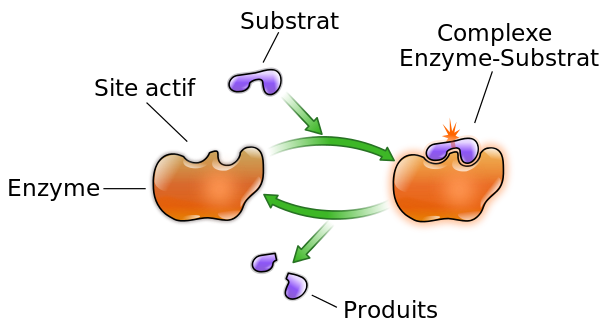
\includegraphics[width=0.6\linewidth]{chimie/cinetique/cinetique.png}
         \caption{Mécanisme clé-serrure}
         \label{fig:my_label}
     \end{figure}
     
     On notera [E$^\ast$] la concentration du complexe enzyme-substrat, [E] la concentration d'enzyme, [S] la concentration du substrat et [P] la concentration du produit.
     
\end{EnvUplevel}

\question En vous inspirant de la Figure 1, proposer un mécanisme en deux étapes modélisant la réaction. \\ On considérera que les deux étapes, notées 1 et 2, sont élémentaires, réversibles et de constantes $k_1$, $k_{-1}$ et $k_2$, $k_{-2}$.
    
\question Caractériser l'équilibre de la réaction S = P.

\question En notant $v(t)$ la vitesse de production de P, donner la loi de vitesse dans l'AEQS en fonction des concentrations [S]$_t$ et [P]$_t$, de la concentration totale en enzyme [E]$_\text{tot}$ = [E]$_t$ + [E$^\ast$]$_t$ et des constantes cinétiques.

\paragraph{Aide :} on pourra chercher la valeur de $\dfrac{[\text{E}]}{[\text{E}]^\ast}$ dans le cadre de l'AEQS et en déduire $\dfrac{[\text{E}]}{[\text{E}]_\text{tot}}$ et  $\dfrac{[\text{E}^\ast]}{[\text{E}]_\text{tot}}$.

\question \'Evaluer les vitesses maximales dans le sens S $\rightarrow$ P et P $\rightarrow$ S.

\question En déduire que la loi de vitesse peut s'écrire
$$v(t) = \dfrac{k_1 v^\text{max}_{\text{S} \rightarrow \text{P}}[\text{S}] - k_{-2} v^\text{max}_{\text{P} \rightarrow \text{S}}[\text{P}]}{k_1(c_\text{s} + [\text{S}]) + k_{-2}(c_\text{p} + [\text{P}])},$$
où $c_\text{s}$ et $c_\text{p}$ sont les deux constantes dites de Michaelis dont on donnera les expressions.

Donner un sens chimique à cette expression.

\uplevel{On se place désormais dans le cas où l'étape donnant le produit est perçue comme irréversible.}

\question Interpréter chimiquement ce que cela signifie à partir de la loi de vitesse de la question 4 et de la constante d'équilibre de la question 3.

\question En déduire une expression simplifiée de la loi de vitesse de la question 6, dépendant uniquement de $v^\text{max}_{\text{S} \rightarrow \text{P}}$ et $c_\text{s}/[\text{S}]$.

\question Etablir une méthode graphique pour évaluer $v_\text{max}$ et $c_\text{s}$.

\end{questions}

\end{exercise}


% Niveau :      PCSI *
% Discipline :  Cinétique
% Mots clés :   Stéréochimie

\begin{exercise}{Modèle épidémiologique}{2}{PCSI}
{Transformationn de la matière,Cinétique}{bermu}

\begin{questions}
\questioncours Notion d'ordre d'une réaction : ordre global, ordre apparent, ordre initial.

\begin{EnvUplevel}
    On s'intéresse à la cinétique de la propagation d'un pathogène dans une population. Pour cela, on divise la population en quatre catégories :
    \begin{itemize}
        \item \textsfbf{S} : les personnes susceptibles d'être contaminées ;
        \item \textsfbf{E} : les personnes exposées au pathogène, en période d'incubation ;
        \item \textsfbf{I} : les personnes infectées et donc contagieuses ;
        \item \textsfbf{R} : les personnes rétablies.
    \end{itemize}
    
    On écrit par ailleurs les processus d'exposition (1), d'infection (2) et de rétablissement (3) comme :
    $$\text{(1)}\quad\textsfbf{S} + \textsfbf{I} \xrightarrow[]{\ \beta\ } \textsfbf{E} + \textsfbf{I}, \qquad\qquad
    \text{(2)}\quad\textsfbf{E} \xrightarrow[]{\ \sigma\ }
      \textsfbf{I} , \qquad\qquad
      \text{(3)}\quad\textsfbf{I}\xrightarrow[]{\ \gamma\ }
      \textsfbf{R} $$
\end{EnvUplevel}

\question Interpréter les réactions (1), (2) et (3) d'un point de vue chimique.

\question En supposant les ordres courants de chaque réaction égaux à la molécularité de chaque espèce, donner la vitesse de chaque réaction en fonction des dérivées $\dv{[\textsfbf{S}]}{t}$, ...

\question En faisant l'approximation des états quasi-stationnaire sur \textsfbf{E}, donner la 


\end{questions}


\end{exercise}


% Niveau :      PCSI *
% Discipline :  Chimie Orga
% Mots clés :   Stéréochimie

\begin{exercise}{Horloge chimique}{3}{PCSI}
{Transformationn de la matière,Cinétique,Arrhénius}{bermu}

\begin{questions}
\questioncours Approximation de l’étape cinétiquement déterminante. \\ On illustrera par un exemple.

\begin{EnvUplevel}
     Hans Heinrich Landolt découvre en 1886 une réaction qu'il qualifie d'horloge chimique.
     
     Partant d'une solution contenant des ions iodure (I$^-$, $\mathrm{[I]_i} = 10$ mmol) et thiosulfate (S$_2$O$_3^{2-}$, $\mathrm{[S_2O_3^{2-}]_i} = 10$ mmol) et de l'amidon (noté L, $\mathrm{[L]_i} = 100$ mmol), on ajoute de l'eau oxygénée (H$_2$O$_2$) acidifiée (H$^+$). Les variations de volumes sont négligées.
     
     On observe que la solution, limpide initialement, devient violette au bout de $\tau = 5$ secondes.
     
     Il se produit trois réactions :
     \begin{enumerate}[label={\quad(\arabic*)}]
         \item $\mathrm{3 I^- + H_2O_2 + 2 H^+ \quad\longrightarrow\quad I_3^- + 2 H_2O}$, lente, $K^\circ_1 = 10^{30}$ ;
         \item entre I$_3^-$ et S$_2$O$_3^{2-}$ qui produit I$^-$ et S$_4$O$_6^{2-}$, rapide, $K^\circ_2 = 10^{50}$ ;
         \item $\mathrm{I_3^- + L \quad\rightleftharpoons\quad [I_3L]^-}$, qui colore la solution en violet, rapide, $K^\circ_3 = 10^{20}$.
     \end{enumerate}
\end{EnvUplevel}

\question Initialement, à $t=0$, seule la réaction (1) se produit.
\begin{parts}
    \part Que veux-t-on dire par 'la réaction est totale et lente' ? Donner des critères quantifiant ces deux affirmations.
    \part Sachant que la concentration en eau oxygénée et en ions H$^+$ est très grande (on précisera devant quoi), donner une expression simplifiée de la loi de vitesse de la réaction 1. On pourra considérer qu'elle est d'ordre effectif 1.
    \part Donner la concentration de $\mathrm{[I_3^-]_1}(t)$ en fonction du temps, et des données du problème, compte tenu uniquement de la réaction (1). Estimer  la constante de vitesse de réaction effective $k^\text{eff}_1$ ainsi que la vitesse de réaction initiale $v^\text{i}_1$ à l'aide des données du problème.
\end{parts}

\question On considère qu'il s'est initialement formé par la réaction (1) une petite quantité $\varepsilon$ de I$_3^-$. \\
Il est immédiatement consommé par les réactions (2) et (3). 
\begin{parts}
    \part Équilibrer l'équation de réaction de (2).
    \part En précisant les hypothèses utilisées et en les justifiant par des calculs rigoureux, donner l'état final du système à l'instant $t$.
    
    % \textsfbf{Aide :} considérer le rapport des avancements volumiques $\xi_2^\text{i,éq}/\xi_3^\text{i,éq}$ à l'instant initial.
    
    \part Comment évolue donc le système initialement ? Donner l'évolution (totale) de $\mathrm{[I^-]}(t)$, $\mathrm{[I_3^-]}(t)$ et $\mathrm{[S_2O_3^{2-}]}(t)$ en fonction des données du problème et de $v_1^\text{i}$.
\end{parts}


\end{questions}

\end{exercise}
